%%---------------------------------------------------------------------------%%
%% adding.tex
%%
%% how to add a new package to the draco system
%%---------------------------------------------------------------------------%%

\chapter{Adding a Package to Draco\index{Draco!adding packages}}
\label{chap:adding}

\section{Overview}
\label{sec:adding_overview}

New \draco\ packages get added in subdirectories under
\comp{draco/src/}.  Each \draco\ package may have its own additional
subdirectories under \comp{draco/src/\vble{pkg}}.
Figure~\ref{fig:package} illustrates a representative package
\begin{figure}[htbp]
  \begin{center}
    \includegraphics[width=2.5in]{fig/package.eps}
    \caption{Standard package directory configuration in \draco.}
    \label{fig:package}
  \end{center}
\end{figure}
directory.  A package directory should conform to following
guidelines:
\begin{itemize}
\item each package directory should have a \comp{test/} subdirectory
    that holds component test code, these tests are also used to
    verify package builds as described in \S~\ref{sec:building_draco}.
\item all subdirectories in the package should have the same
  configuration and build options,
\item packages should use the \draco\ system default
  \comp{Makefile.package.in}\index{Makefile.package.in} and
  \comp{Makefile.test.in}\index{Makefile.test.in} makefiles,
\item packages should use the \draco\ system default \autoconf\ macros
  in \comp{aclocal.m4}\index{aclocal.m4} in
  \comp{configure.in}\index{configure.in|(},
\item if the package has special needs, it can have a unique
  \comp{Makefile.in}\index{Makefile.in|(},
\item special configuration requirements for a package may be added to 
  that package's \comp{configure.in} file.
\end{itemize}
In general, most packages will be able to use the default makefiles
and configure templates that are provided by \draco.  Customization of 
package configure files is treated in \S~\ref{sec:customize}.

At a minimum, each package requires a
\comp{configure.in} file to produce a
\comp{configure*} script.  Additionally, the package must have access
to a makefile template.  \draco\ provides the default makefile
templates \comp{Makefile.package.in} and
\comp{Makefile.test.in} for
\comp{src/\vble{pkg}/} and \comp{src/\vble{pkg}/test} directories.
Finally, to set configuration options on a package-by-package basis,
the files \comp{config.h.in}\index{config.h.in|(} and
\comp{\vble{pkg}-\vble{vendor}.h}\index{pkg-vendor.h|(} are required.
Table~\ref{tab:pkgfiles} lists all of the possible configuration files
\begin{table}
  \caption{\draco\ build system package files.}
  \label{tab:pkgfiles}
  \begin{center}
    \begin{tabularx}{\linewidth}{
        >{\setlength{\hsize}{.5\hsize}}L %
        >{\setlength{\hsize}{1.5\hsize}}X}
      \hline\hline
      \multicolumn{1}{Y}{Package Configuration Files} &  
      \multicolumn{1}{Y}{Description} \\
      \hline
                                % configure.in
      configure.in & file containing \autoconf\ tests that is used to
      build \comp{configure*} \\
                                % configure*
      configure* & package configure script generated by \autoconf\ from 
      \comp{configure.in} \\
                                % Makefile.in
      Makefile.in & special package makefile, this is present only if
      the default \comp{Makefile.package.in} is not used \\
                                % Makefile.srcs
      Makefile.srcs & special source modifications, called by the
      default makefiles \\
                                % Makefile.target
      Makefile.target & special target modifications for package test
      directories, called by the default makefiles \\
                                % Makefile.misc
      Makefile.misc & special makefile for miscellaneous additions,
      called by the default makefiles \\
                                % config.h.in
      config.h.in & package specific environment configuration file \\
                                % package-vendor.h
      \vble{pkg}-\vble{vendor}.h & package-specific vendor include
      headers \\
      \hline\hline
    \end{tabularx}
  \end{center}
\end{table}
that can be found in a \draco\ package.  All of these files are
explained in \S~\ref{sec:package_files}.

\draco\ provides templates for package-level \comp{configure.in} and
\comp{Makefile.in} files.  \draco\ templates are located in two places
in the \draco\ source tree, \comp{draco/config} and
\comp{draco/templates}.  Figure~\ref{fig:src_draco} shows the contents
of these directories.  Table~\ref{tab:templates} gives a description
\begin{table}
  \caption{\draco\ build system templates.}
  \label{tab:templates}
  \begin{center}
    \begin{tabularx}{\linewidth}{
        >{\setlength{\hsize}{.85\hsize}}L %
        >{\setlength{\hsize}{.65\hsize}}L %
        >{\setlength{\hsize}{1.5\hsize}}X}
      \hline\hline
      \multicolumn{1}{Y}{Template File} & \multicolumn{1}{Y}{Location} 
      & \multicolumn{1}{Y}{Description} \\
      \hline
                                % Makefile.package.in
      Makefile.package.in & draco/config & default makefile template
      for \draco\ packages \\
                                % Makefile.test.in
      Makefile.test.in & draco/config & default makefile template for
      \draco\ package \comp{test/} directories \\
                                % configure.package.in
      configure.package.in & draco/templates & standard
      \comp{configure.in} template for \draco\ packages \\
                                % template.h
      template.h & draco/templates & template for \cc\ header files,
      both \comp{*.h} and \comp{*.h.in} headers \\
                                % template.hh
      template.hh & draco/templates & template for \cpp\ header files,
      both \comp{*.hh} and \comp{*.hh.in} headers \\
                                % template.cc
      template.cc & draco/templates & template for \cpp\ implementation
      and explicit instantiation files \\
                                % template.t.hh
      template.t.hh & draco/templates & template for \cpp\ templated
      code \\
      \hline\hline
    \end{tabularx}
  \end{center}
\end{table}
of each template file.

\draco\ macros are defined in \comp{draco/config/aclocal.m4}.  These
macros are used by \autoconf\ to generate the tests that go into
\comp{configure*} scripts.  The macros are divided into two basic
categories: (a) macros used in \comp{configure.in}, (b) macros used
internally in \comp{aclocal.m4}.  In general, \draco\ package
developers need only be concerned with (a).  These are summarized in
\S~\ref{sec:package_files}.  The macros in category (b) are the domain
of \draco\ system developers and are described in
Chap.~\ref{chap:extend}.

Most package directories use the default makefile templates in
\comp{draco/config}.  These are called from the package's
\comp{configure.in} script; thus, they are not seen inside of the
package directory.  Simple modifications to the standard makefiles is
achieved by adding \comp{Makefile.srcs}, \comp{Makefile.targets},
and/or \comp{Makefile.misc}.  The use of these files is summarized in
\S~\ref{sec:package_files}. 

In summary, each package has a \comp{test/} directory for component
tests.  Additional subdirectories that contain package components may
be included.  All package subdirectories are configured using the same
options.  Packages may define unique macros inside of
\comp{src/\vble{pkg}/configure.in}.  Also, packages may use a unique
\comp{Makefile.in} if they require special functionality that does not
exist in the standard makefile templates.  We will now turn our
attention to a more detailed description of the configure files.

%%---------------------------------------------------------------------------%%

\section{Package Files}
\label{sec:package_files}

In this section we give expanded descriptions of the default
package-dependent files listed in Table~\ref{tab:pkgfiles}.  We will
not go into great detail about the \autoconf\ macros and default
makefiles that are defined in the \draco\ system.  That discussion is
reserved until Chap.~\ref{chap:extend}.  We will concentrate primarily
on the three file-types that are found in each package directory:
\comp{configure.in}, \comp{config.h.in}, and
\comp{\vble{pkg}-vendor.h}.  We reserve a discussion of makefile
customization until \S~\ref{sec:customize}.
\begin{description}
\item[\comp{configure.in}]\index{configure.in|textbf} The
  \comp{configure.in} file determines how the \comp{configure*} script
  gets built by \autoconf.  We will step through a standard package
  \comp{configure.in} script to learn how to generate package
  \comp{configure*} files.  Consider the \cfour\ \comp{configure.in}
  script illustrated in Fig.~\ref{fig/c4-in}.
  \cdFramedFigure{fig/c4-in}{\comp{configure.in} file in the \textsc{c4}
    package.}
\end{description}

%%---------------------------------------------------------------------------%%

\section{Customized Packages}
\label{sec:customize}

%%---------------------------------------------------------------------------%%
%% indices

\index{configure.in|)}
\index{Makefile.in|)}
\index{config.h.in|)}
\index{pkg-vendor.h|)}

%%---------------------------------------------------------------------------%%

